\begin{center}
    {\LARGE \textbf{2025有机化学与分析化学}} \\[2ex]
    {\large 时量180分钟 \quad 满分150分}
\end{center}

\vspace{0.5cm}
\noindent\textbf{注意事项:}
\begin{enumerate}[label=\arabic*., parsep=0pt, itemsep=0pt]
    \item 答题前,考生先将自己的姓名、学号、考场号、座位号填写在答题卡上,将条形码准确粘贴在考生信息条形码粘贴区。
    \item 考试结束后,将本试卷与答题纸一并收回。
    \item 回答各个问题时,将答案写在答题纸上,写在本试卷上无效。
\end{enumerate}

\vspace{1cm}
\begin{center}
    {\Large \textbf{有机化学部分(共100分)}}
\end{center}

\vspace{0.5cm}
\noindent\textbf{一、选择题（15 pts.）}

\begin{enumerate}[label=\arabic*., itemsep=1.5ex]
    \item 缺失
\end{enumerate}

\vspace{0.5cm}
\noindent\textbf{二、完成反应(29 pts.)}

\begin{enumerate}[label=\arabic*., itemsep=3ex]
    \item 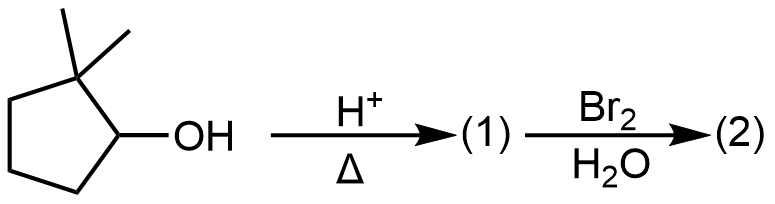
\includegraphics[scale=0.3, valign=c]{./Figure/2025/2025_1_1.png} 
    \item 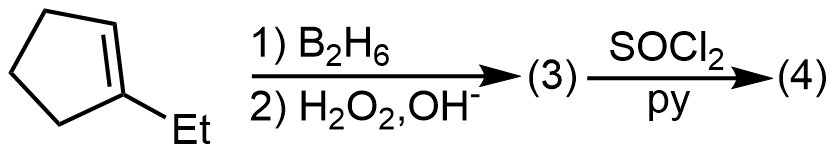
\includegraphics[scale=0.3, valign=c]{./Figure/2025/2025_1_2.png}
    \item 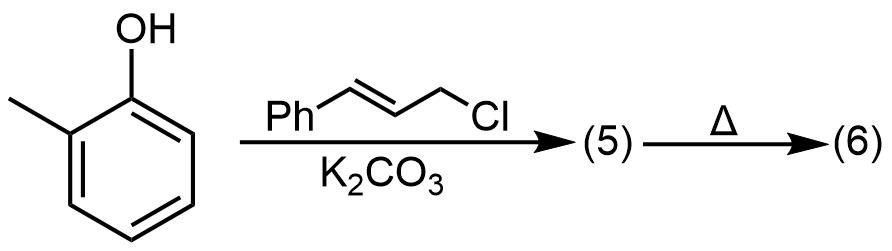
\includegraphics[scale=0.3, valign=c]{./Figure/2025/2025_1_3.png}
    \item 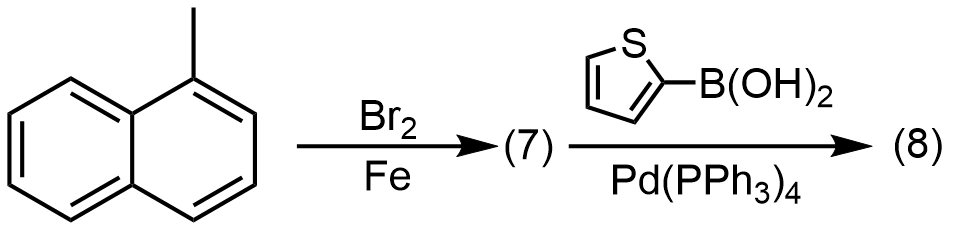
\includegraphics[scale=0.3, valign=c]{./Figure/2025/2025_1_4.png}
    \item 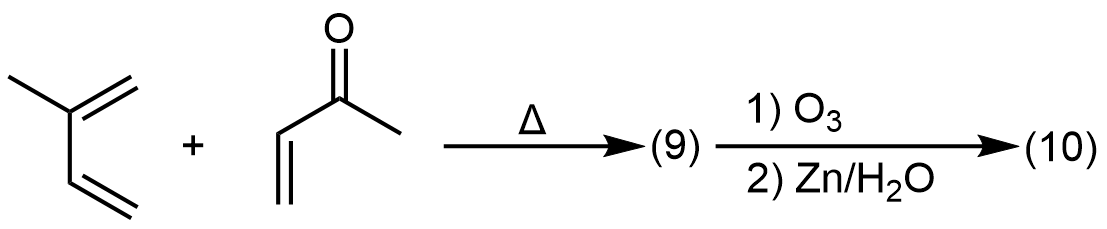
\includegraphics[scale=0.3, valign=c]{./Figure/2025/2025_1_5.png}
    \item 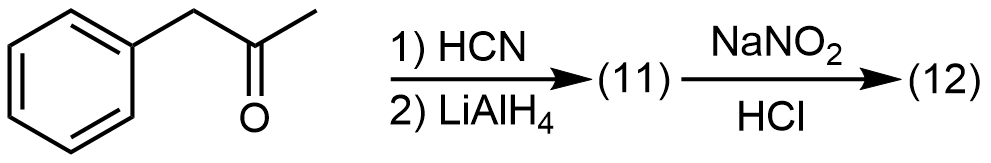
\includegraphics[scale=0.3, valign=c]{./Figure/2025/2025_1_6.png}
    \item 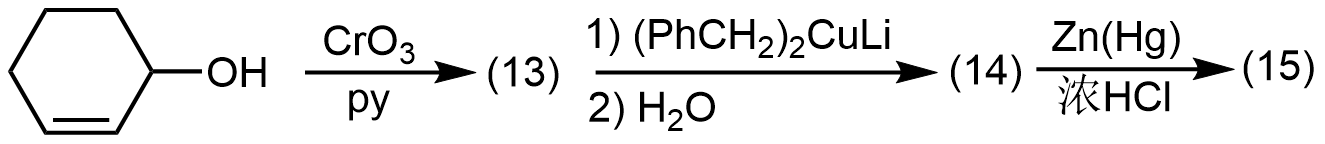
\includegraphics[scale=0.3, valign=c]{./Figure/2025/2025_1_7.png}
    \item 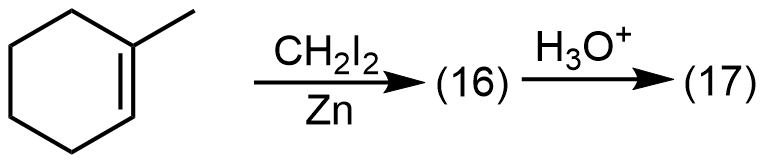
\includegraphics[scale=0.3, valign=c]{./Figure/2025/2025_1_8.png}
    \item 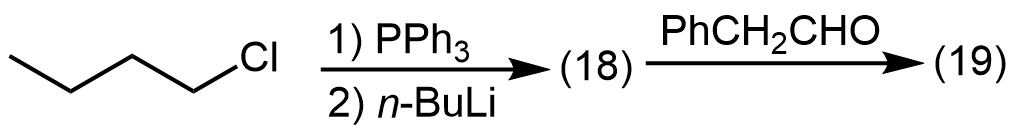
\includegraphics[scale=0.3, valign=c]{./Figure/2025/2025_1_9.png}
    \item 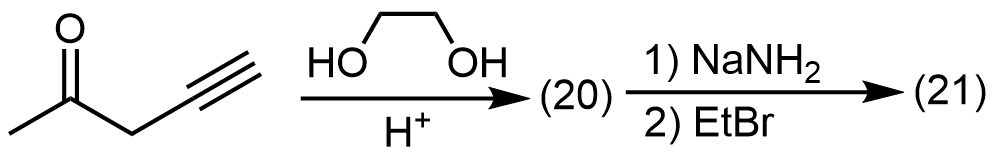
\includegraphics[scale=0.3, valign=c]{./Figure/2025/2025_1_10.png}
    \item 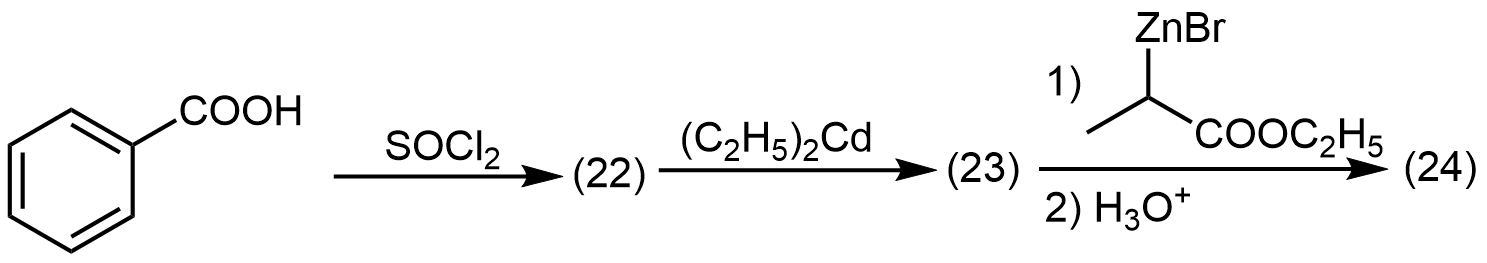
\includegraphics[scale=0.3, valign=c]{./Figure/2025/2025_1_11.png}
    \item 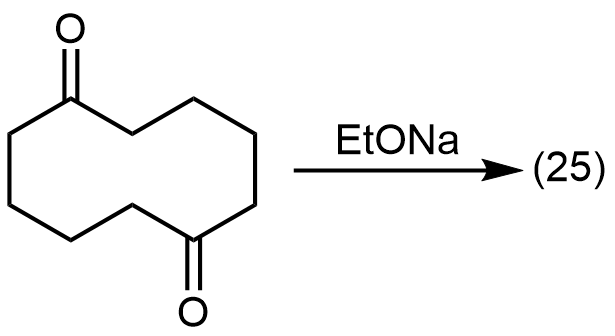
\includegraphics[scale=0.3, valign=c]{./Figure/2025/2025_1_12.png}
    \item 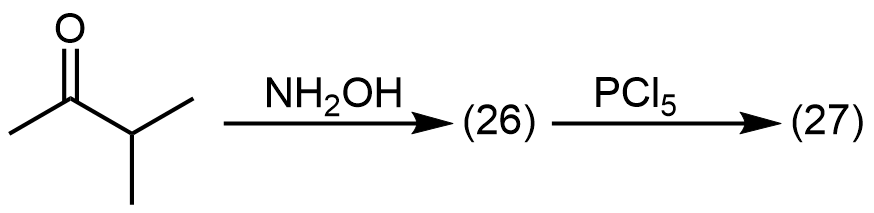
\includegraphics[scale=0.3, valign=c]{./Figure/2025/2025_1_13.png}
    \item 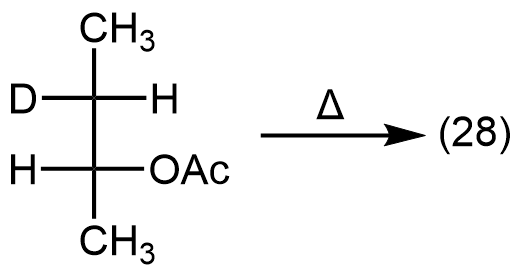
\includegraphics[scale=0.3, valign=c]{./Figure/2025/2025_1_14.png}
    \item 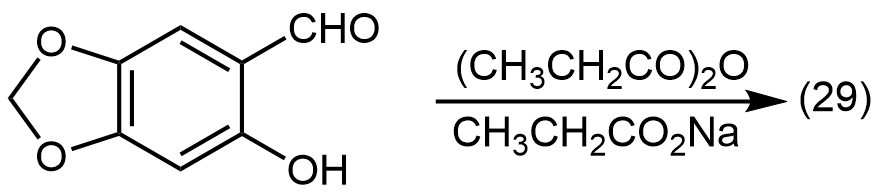
\includegraphics[scale=0.3, valign=c]{./Figure/2025/2025_1_15.png}

\end{enumerate}

\vspace{0.5cm}
\noindent\textbf{三、简答题(7 pts.)}

\begin{enumerate}[label=\arabic*., itemsep=3ex]
    \item 解释薁(Azulene)在 1-位发生亲电取代反应，在 4,6-位发生亲核取代反应的原因.
    
    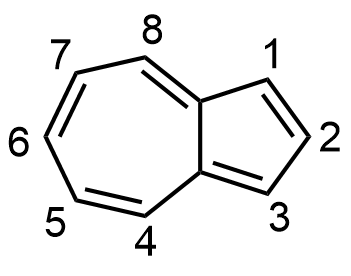
\includegraphics[scale=0.3, valign=c]{./Figure/2025/2025_5_1.png}
\end{enumerate}


\vspace{0.5cm}
\noindent\textbf{四、机理题(14 pts.)}

\begin{enumerate}[label=\arabic*., start=1, itemsep=1.5ex]
    \item 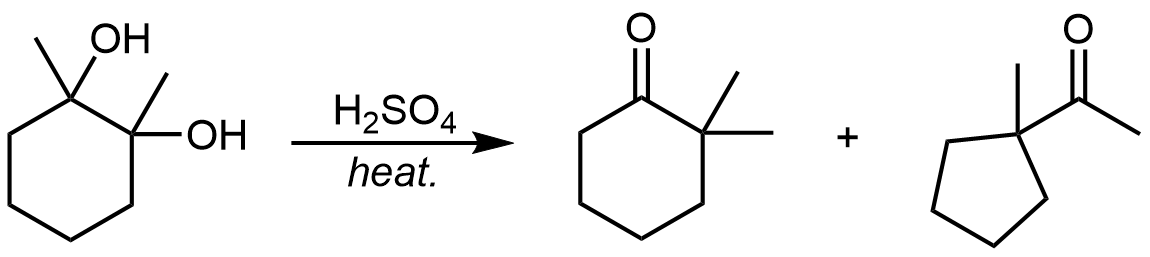
\includegraphics[scale=0.3, valign=c]{./Figure/2025/2025_2_1.png}
    \item 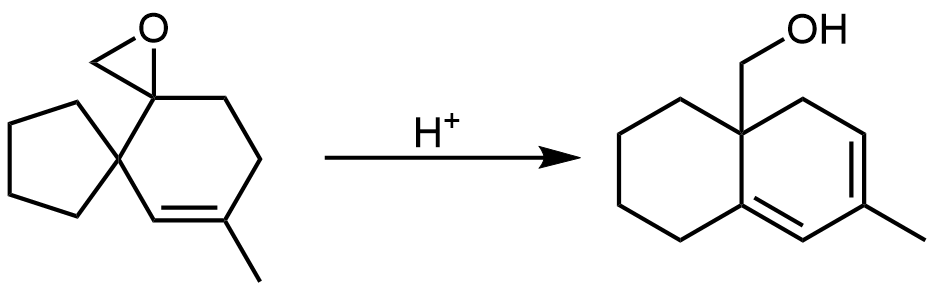
\includegraphics[scale=0.3, valign=c]{./Figure/2025/2025_2_2.png}

\end{enumerate}

\vspace{0.5cm}
\noindent\textbf{五、合成题(35 pts.)}

\begin{enumerate}[label=\arabic*., start=1, itemsep=1.5ex]

    \begin{figure}[htbp]
        \centering
        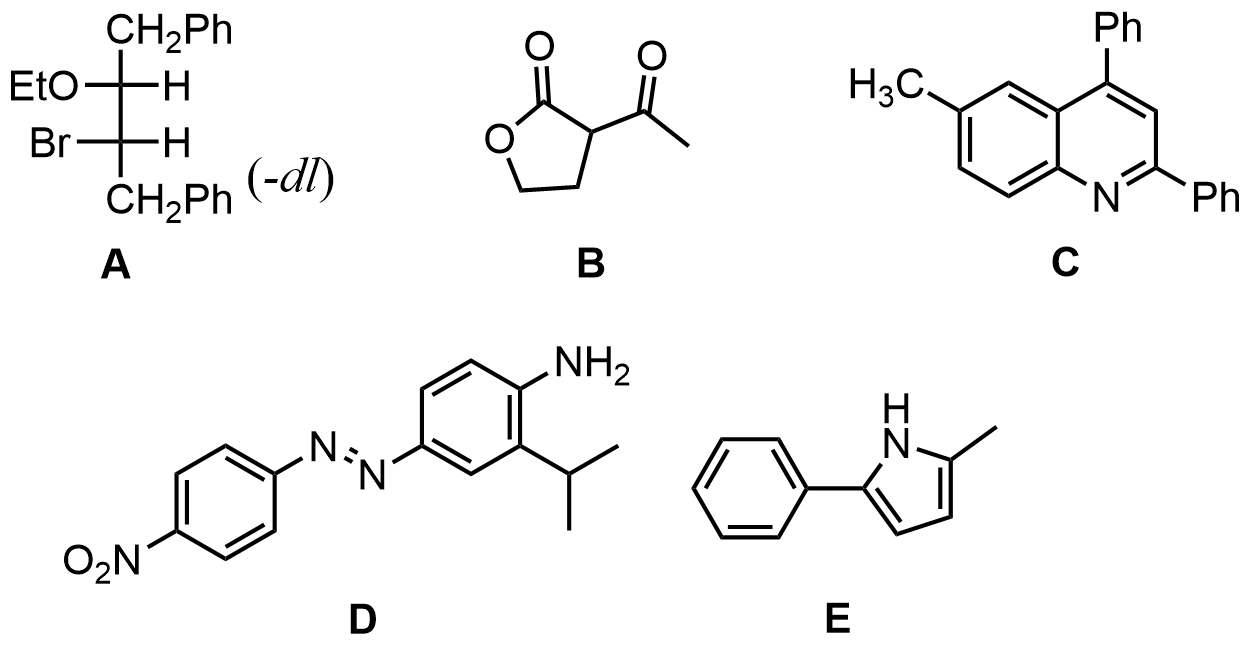
\includegraphics[scale=0.38]{./Figure/2025/2025_3.png}
    \end{figure}
    \item 以苯和乙炔为主要有机原料合成化合物\textbf{A}
    \item 以不超过两个碳原子的有机原料合成化合物\textbf{B}
    \item 以苯和不超过两个碳原子的有机原料合成化合物\textbf{C}
    \item 以苯和不超过三个碳原子的有机原料合成化合物\textbf{D}
    \item 以苯不超过三个碳原子的有机原料合成化合物\textbf{E}
\end{enumerate}

\vspace{1cm}
\begin{center}
    {\Large \textbf{分析化学部分(共50分)}}
\end{center}

\vspace{0.5cm}
\noindent\textbf{六、简答题：简要回答下列问题。本题共 5 小题，每小题 4 分，共 20 分。}

\begin{enumerate}[label=\arabic*., itemsep=1.5ex]
    \item 标定盐酸时使用以下两种基准物质，无水碳酸钠，十水合硼砂，据此回答下列问题并解释原因：
    \begin{enumerate}[label=(\arabic*), noitemsep, topsep=0pt, partopsep=0pt]
        \item 请判断以下情况对盐酸的标定有何影响？
        \begin{enumerate}[label=\alph*., noitemsep, topsep=0pt, partopsep=0pt]
            \item $\ce{Na2CO3}$ 中吸收少量水分
            \item 硼砂失去少量结晶水
        \end{enumerate}
        \item 若不存在上述误差，且操作过程完全正确，标定盐酸时，用何种物质较好？
    \end{enumerate}

    \item 根据 $\ce{K2Cr2O7}$ 法测定铁含量的实验回答下列问题：
    \begin{enumerate}[label=(\arabic*), noitemsep, topsep=0pt, partopsep=0pt]
        \item 加入稍过量 $\ce{SnCl2}$ 的目的是什么？为什么不能加入太多 $\ce{SnCl2}$？
        \item 体系中使用硫磷混酸的作用是什么？
        \item 实验使用了指示剂二苯胺磺酸钠，该指示剂氧化态和还原态的颜色分别为？
    \end{enumerate}

    \item EDTA 可以连续测定样品中的 $\ce{Bi^{3+}}$ 和 $\ce{Pb^{2+}}$ 含量。选用二甲酚橙(XO)为指示剂，先在 $\text{pH}=1$ 介质中滴定 $\ce{Bi^{3+}}$，然后加入六亚甲基四胺调节 $\text{pH}$ 至 5，滴定 $\ce{Pb^{2+}}$。已知 $\lg K_{\ce{BiY}}$ 和 $\lg K_{\ce{PbY}}$ 分别为 27.94 和 18.04。
    \begin{enumerate}[label=(\arabic*), noitemsep, topsep=0pt, partopsep=0pt]
        \item 滴定 $\ce{Bi^{3+}}$ 时酸度过高或过低对结果有何影响？
        \item 为什么要调节 $\text{pH}$ 至 5？能否使用 $\ce{NaAc}$ 或者 $\ce{NH3\cdot H2O}$ 的缓冲溶液？
        \item 全滴定过程中体系的颜色如何变化？分别对应哪一阶段？
    \end{enumerate}

    \item （判断有无系统误差的题，用 $t = \frac{|\mu - \bar{x}|}{s}\sqrt{n}$，均值和方差都已给出，不用计算）

    \item 根据下表所给数据，填写下列表格中的空缺值：
    \begin{center}
    \begin{tabular}{|l|c|c|c|}
    \hline
    滴定体系 & 计量点前 $1\%$ & 计量点 & 计量点后 $1\%$ \\
    \hline
    $\ce{Ce^{4+}}$ 滴定 $\ce{Fe^{2+}}$ & $0.86$ & $1.06$ & \\
    \hline
    $\ce{Fe^{3+}}$ 滴定 $\ce{Sn^{2+}}$ & & $0.32$ & $0.50$ \\
    \hline
    \end{tabular}
    \end{center}
\end{enumerate}

\vspace{0.5cm}
\noindent\textbf{七、解答题：解答应给出详细步骤。本题共 3 小题，每小题 10 分，共 30 分。}

\begin{enumerate}[label=\arabic*., itemsep=1.5ex]
    \item 用 $0.20\,\mathrm{mol/L}$ 的 $\ce{NaOH}$ 溶液滴定同浓度的甲酸($\ce{HA}$)溶液，已知 $\text{p}K_{\text{a}}(\ce{HA})=3.74$。
    \begin{enumerate}[label=(\arabic*), noitemsep, topsep=0pt, partopsep=0pt]
        \item 求化学计量点的 $\text{pH}$ 及滴定突跃范围。
        \item 当 $\text{pH}_{\text{ep}}=7.0$ 时，计算终点误差。
    \end{enumerate}

    \item 计算 $\ce{PbSO4}$ 在纯水以及 $1\,\mathrm{mol/L}$ 的 $\ce{HCl}$ 溶液中的溶解度。
    \\
    已知：$\ce{H2SO4}$ 的 $\text{p}K_{a2}=2$；$\ce{Pb-Cl}$ 配合物的 $\lg\beta_1\sim\lg\beta_3$ 分别为 $1.2$、$0.6$、$1.2$；$\ce{PbSO4}$ 的 $\lg K_{\text{sp}}=-8.0$；不考虑盐效应。

    \item 在 $\text{pH}=5.5$ 的缓冲溶液中，用 $0.020\,\mathrm{mol/L}$ 的 EDTA 标准溶液滴定含有 $0.020\,\mathrm{mol/L}$ 的 $\ce{Al^{3+}}$ 和 $\ce{Pb^{2+}}$ 混合液中的 $\ce{Pb^{2+}}$，采用二甲酚橙(XO)作为指示剂。在溶液中加入固体 $\ce{NH4F}$（假定 $\text{pH}$ 保持不变），至平衡时 $[\ce{F^-}]=0.01\,\mathrm{mol/L}$，计算确定掩蔽效果以及终点误差。
    \\
    已知：$\lg K_{\ce{AlY}}=16.3$，$\lg K_{\ce{PbY}}=18.0$；$\text{pH}=5.5$ 时，$\text{pPb}_{\text{ep}}(\text{XO})=7.6$，$\lg\alpha_{Y(\text{H})}=5.5$，$\alpha_{\ce{Al(OH)}}=0.4$；$\ce{Al-F}$ 配合物的 $\lg\beta_1\sim\lg\beta_6$ 分别为 $6.1$、$11.2$、$15.0$、$17.7$、$19.4$、$19.7$。
\end{enumerate}